% Options for packages loaded elsewhere
\PassOptionsToPackage{unicode}{hyperref}
\PassOptionsToPackage{hyphens}{url}
\PassOptionsToPackage{dvipsnames,svgnames,x11names}{xcolor}
%
\documentclass[
  letterpaper,
  DIV=11,
  numbers=noendperiod]{scrartcl}

\usepackage{amsmath,amssymb}
\usepackage{iftex}
\ifPDFTeX
  \usepackage[T1]{fontenc}
  \usepackage[utf8]{inputenc}
  \usepackage{textcomp} % provide euro and other symbols
\else % if luatex or xetex
  \usepackage{unicode-math}
  \defaultfontfeatures{Scale=MatchLowercase}
  \defaultfontfeatures[\rmfamily]{Ligatures=TeX,Scale=1}
\fi
\usepackage{lmodern}
\ifPDFTeX\else  
    % xetex/luatex font selection
\fi
% Use upquote if available, for straight quotes in verbatim environments
\IfFileExists{upquote.sty}{\usepackage{upquote}}{}
\IfFileExists{microtype.sty}{% use microtype if available
  \usepackage[]{microtype}
  \UseMicrotypeSet[protrusion]{basicmath} % disable protrusion for tt fonts
}{}
\makeatletter
\@ifundefined{KOMAClassName}{% if non-KOMA class
  \IfFileExists{parskip.sty}{%
    \usepackage{parskip}
  }{% else
    \setlength{\parindent}{0pt}
    \setlength{\parskip}{6pt plus 2pt minus 1pt}}
}{% if KOMA class
  \KOMAoptions{parskip=half}}
\makeatother
\usepackage{xcolor}
\setlength{\emergencystretch}{3em} % prevent overfull lines
\setcounter{secnumdepth}{2}
% Make \paragraph and \subparagraph free-standing
\ifx\paragraph\undefined\else
  \let\oldparagraph\paragraph
  \renewcommand{\paragraph}[1]{\oldparagraph{#1}\mbox{}}
\fi
\ifx\subparagraph\undefined\else
  \let\oldsubparagraph\subparagraph
  \renewcommand{\subparagraph}[1]{\oldsubparagraph{#1}\mbox{}}
\fi

\usepackage{color}
\usepackage{fancyvrb}
\newcommand{\VerbBar}{|}
\newcommand{\VERB}{\Verb[commandchars=\\\{\}]}
\DefineVerbatimEnvironment{Highlighting}{Verbatim}{commandchars=\\\{\}}
% Add ',fontsize=\small' for more characters per line
\usepackage{framed}
\definecolor{shadecolor}{RGB}{241,243,245}
\newenvironment{Shaded}{\begin{snugshade}}{\end{snugshade}}
\newcommand{\AlertTok}[1]{\textcolor[rgb]{0.68,0.00,0.00}{#1}}
\newcommand{\AnnotationTok}[1]{\textcolor[rgb]{0.37,0.37,0.37}{#1}}
\newcommand{\AttributeTok}[1]{\textcolor[rgb]{0.40,0.45,0.13}{#1}}
\newcommand{\BaseNTok}[1]{\textcolor[rgb]{0.68,0.00,0.00}{#1}}
\newcommand{\BuiltInTok}[1]{\textcolor[rgb]{0.00,0.23,0.31}{#1}}
\newcommand{\CharTok}[1]{\textcolor[rgb]{0.13,0.47,0.30}{#1}}
\newcommand{\CommentTok}[1]{\textcolor[rgb]{0.37,0.37,0.37}{#1}}
\newcommand{\CommentVarTok}[1]{\textcolor[rgb]{0.37,0.37,0.37}{\textit{#1}}}
\newcommand{\ConstantTok}[1]{\textcolor[rgb]{0.56,0.35,0.01}{#1}}
\newcommand{\ControlFlowTok}[1]{\textcolor[rgb]{0.00,0.23,0.31}{#1}}
\newcommand{\DataTypeTok}[1]{\textcolor[rgb]{0.68,0.00,0.00}{#1}}
\newcommand{\DecValTok}[1]{\textcolor[rgb]{0.68,0.00,0.00}{#1}}
\newcommand{\DocumentationTok}[1]{\textcolor[rgb]{0.37,0.37,0.37}{\textit{#1}}}
\newcommand{\ErrorTok}[1]{\textcolor[rgb]{0.68,0.00,0.00}{#1}}
\newcommand{\ExtensionTok}[1]{\textcolor[rgb]{0.00,0.23,0.31}{#1}}
\newcommand{\FloatTok}[1]{\textcolor[rgb]{0.68,0.00,0.00}{#1}}
\newcommand{\FunctionTok}[1]{\textcolor[rgb]{0.28,0.35,0.67}{#1}}
\newcommand{\ImportTok}[1]{\textcolor[rgb]{0.00,0.46,0.62}{#1}}
\newcommand{\InformationTok}[1]{\textcolor[rgb]{0.37,0.37,0.37}{#1}}
\newcommand{\KeywordTok}[1]{\textcolor[rgb]{0.00,0.23,0.31}{#1}}
\newcommand{\NormalTok}[1]{\textcolor[rgb]{0.00,0.23,0.31}{#1}}
\newcommand{\OperatorTok}[1]{\textcolor[rgb]{0.37,0.37,0.37}{#1}}
\newcommand{\OtherTok}[1]{\textcolor[rgb]{0.00,0.23,0.31}{#1}}
\newcommand{\PreprocessorTok}[1]{\textcolor[rgb]{0.68,0.00,0.00}{#1}}
\newcommand{\RegionMarkerTok}[1]{\textcolor[rgb]{0.00,0.23,0.31}{#1}}
\newcommand{\SpecialCharTok}[1]{\textcolor[rgb]{0.37,0.37,0.37}{#1}}
\newcommand{\SpecialStringTok}[1]{\textcolor[rgb]{0.13,0.47,0.30}{#1}}
\newcommand{\StringTok}[1]{\textcolor[rgb]{0.13,0.47,0.30}{#1}}
\newcommand{\VariableTok}[1]{\textcolor[rgb]{0.07,0.07,0.07}{#1}}
\newcommand{\VerbatimStringTok}[1]{\textcolor[rgb]{0.13,0.47,0.30}{#1}}
\newcommand{\WarningTok}[1]{\textcolor[rgb]{0.37,0.37,0.37}{\textit{#1}}}

\providecommand{\tightlist}{%
  \setlength{\itemsep}{0pt}\setlength{\parskip}{0pt}}\usepackage{longtable,booktabs,array}
\usepackage{calc} % for calculating minipage widths
% Correct order of tables after \paragraph or \subparagraph
\usepackage{etoolbox}
\makeatletter
\patchcmd\longtable{\par}{\if@noskipsec\mbox{}\fi\par}{}{}
\makeatother
% Allow footnotes in longtable head/foot
\IfFileExists{footnotehyper.sty}{\usepackage{footnotehyper}}{\usepackage{footnote}}
\makesavenoteenv{longtable}
\usepackage{graphicx}
\makeatletter
\def\maxwidth{\ifdim\Gin@nat@width>\linewidth\linewidth\else\Gin@nat@width\fi}
\def\maxheight{\ifdim\Gin@nat@height>\textheight\textheight\else\Gin@nat@height\fi}
\makeatother
% Scale images if necessary, so that they will not overflow the page
% margins by default, and it is still possible to overwrite the defaults
% using explicit options in \includegraphics[width, height, ...]{}
\setkeys{Gin}{width=\maxwidth,height=\maxheight,keepaspectratio}
% Set default figure placement to htbp
\makeatletter
\def\fps@figure{htbp}
\makeatother

\KOMAoption{captions}{tableheading}
\usepackage{marginnote, here, relsize, needspace, setspace} \def\it{\emph}
\makeatletter
\@ifpackageloaded{caption}{}{\usepackage{caption}}
\AtBeginDocument{%
\ifdefined\contentsname
  \renewcommand*\contentsname{Table of contents}
\else
  \newcommand\contentsname{Table of contents}
\fi
\ifdefined\listfigurename
  \renewcommand*\listfigurename{List of Figures}
\else
  \newcommand\listfigurename{List of Figures}
\fi
\ifdefined\listtablename
  \renewcommand*\listtablename{List of Tables}
\else
  \newcommand\listtablename{List of Tables}
\fi
\ifdefined\figurename
  \renewcommand*\figurename{Figure}
\else
  \newcommand\figurename{Figure}
\fi
\ifdefined\tablename
  \renewcommand*\tablename{Table}
\else
  \newcommand\tablename{Table}
\fi
}
\@ifpackageloaded{float}{}{\usepackage{float}}
\floatstyle{ruled}
\@ifundefined{c@chapter}{\newfloat{codelisting}{h}{lop}}{\newfloat{codelisting}{h}{lop}[chapter]}
\floatname{codelisting}{Listing}
\newcommand*\listoflistings{\listof{codelisting}{List of Listings}}
\makeatother
\makeatletter
\makeatother
\makeatletter
\@ifpackageloaded{caption}{}{\usepackage{caption}}
\@ifpackageloaded{subcaption}{}{\usepackage{subcaption}}
\makeatother
\ifLuaTeX
  \usepackage{selnolig}  % disable illegal ligatures
\fi
\usepackage{bookmark}

\IfFileExists{xurl.sty}{\usepackage{xurl}}{} % add URL line breaks if available
\urlstyle{same} % disable monospaced font for URLs
\hypersetup{
  pdftitle={Lab: Multinomial Regression},
  pdfauthor={KW},
  colorlinks=true,
  linkcolor={blue},
  filecolor={Maroon},
  citecolor={Blue},
  urlcolor={Blue},
  pdfcreator={LaTeX via pandoc}}

\title{Lab: Multinomial Regression}
\usepackage{etoolbox}
\makeatletter
\providecommand{\subtitle}[1]{% add subtitle to \maketitle
  \apptocmd{\@title}{\par {\large #1 \par}}{}{}
}
\makeatother
\subtitle{Princeton University}
\author{KW}
\date{2025-02-26}

\begin{document}
\maketitle

Lab Goal: Predict voting frequency using demographic variables Data
source: FiveThirtyEight ``Why Many Americans Don't Vote'' survey Method:
Multinomial logistic regression

\subsection{Data}\label{data}

The data for this assignment comes from an online Ipsos survey that was
conducted for the FiveThirtyEight article
\href{https://projects.fivethirtyeight.com/non-voters-poll-2020-election/}{``Why
Many Americans Don't Vote''}. You can read more about the survey design
and respondents in the README of the
\href{https://github.com/fivethirtyeight/data/tree/master/non-voters}{GitHub
repo} for the data.

Respondents were asked a variety of questions about their political
beliefs, thoughts on multiple issues, and voting behavior. We will focus
on using the demographic variables and someone's party identification to
understand whether a person is a probable voter.

The variables we'll focus on were (definitions from the codebook in data
set GitHub repo):

\begin{itemize}
\item
  \texttt{ppage}: Age of respondent
\item
  \texttt{educ}: Highest educational attainment category.\\
\item
  \texttt{race}: Race of respondent, census categories. Note: all
  categories except Hispanic were non-Hispanic.
\item
  \texttt{gender}: Gender of respondent
\item
  \texttt{income\_cat}: Household income category of respondent
\item
  \texttt{Q30}: Response to the question ``Generally speaking, do you
  think of yourself as a\ldots{}''

  \begin{itemize}
  \tightlist
  \item
    1: Republican
  \item
    2: Democrat
  \item
    3: Independent
  \item
    4: Another party, please specify
  \item
    5: No preference
  \item
    -1: No response
  \end{itemize}
\item
  \texttt{voter\_category}: past voting behavior:

  \begin{itemize}
  \tightlist
  \item
    \textbf{always}: respondent voted in all or all-but-one of the
    elections they were eligible in
  \item
    \textbf{sporadic}: respondent voted in at least two, but fewer than
    all-but-one of the elections they were eligible in
  \item
    \textbf{rarely/never}: respondent voted in 0 or 1 of the elections
    they were eligible in
  \end{itemize}
\end{itemize}

You can read in the data directly from the GitHub repo:

\begin{Shaded}
\begin{Highlighting}[]
\FunctionTok{library}\NormalTok{(nnet)}
\FunctionTok{library}\NormalTok{(car)}
\FunctionTok{library}\NormalTok{(tidyverse)}
\FunctionTok{library}\NormalTok{(emmeans)}
\FunctionTok{library}\NormalTok{(ggeffects)}
\FunctionTok{library}\NormalTok{(knitr)}
\FunctionTok{library}\NormalTok{(patchwork)}
\FunctionTok{library}\NormalTok{(broom)}
\FunctionTok{library}\NormalTok{(parameters)}
\FunctionTok{library}\NormalTok{(easystats)}
\end{Highlighting}
\end{Shaded}

\begin{Shaded}
\begin{Highlighting}[]
\NormalTok{voter\_data }\OtherTok{\textless{}{-}} \FunctionTok{read\_csv}\NormalTok{(}\StringTok{"https://raw.githubusercontent.com/fivethirtyeight/data/master/non{-}voters/nonvoters\_data.csv"}\NormalTok{)}
\end{Highlighting}
\end{Shaded}

\section{Lab}\label{lab}

\begin{itemize}
\tightlist
\item
  The variable \texttt{Q30} contains the respondent's political party
  identification. Make a new variable that simplifies \texttt{Q30} into
  four categories: ``Democrat'', ``Republican'', ``Independent'',
  ``Other'' (``Other'' also includes respondents who did not answer the
  question).
\end{itemize}

\begin{Shaded}
\begin{Highlighting}[]
\NormalTok{voter\_data }\OtherTok{\textless{}{-}}\NormalTok{ voter\_data }\SpecialCharTok{\%\textgreater{}\%}
  \FunctionTok{mutate}\NormalTok{(}\AttributeTok{pol\_ident\_new =} \FunctionTok{case\_when}\NormalTok{(}
\NormalTok{    Q30}\SpecialCharTok{==}\DecValTok{1} \SpecialCharTok{\textasciitilde{}} \StringTok{"Rep"}\NormalTok{, }
\NormalTok{    Q30}\SpecialCharTok{==}\DecValTok{2} \SpecialCharTok{\textasciitilde{}} \StringTok{"Dem"}\NormalTok{, }
\NormalTok{    Q30}\SpecialCharTok{==}\DecValTok{3} \SpecialCharTok{\textasciitilde{}} \StringTok{"Indep"}\NormalTok{, }
    \ConstantTok{TRUE} \SpecialCharTok{\textasciitilde{}} \StringTok{"Other"}
\NormalTok{  ))}
\end{Highlighting}
\end{Shaded}

\begin{itemize}
\tightlist
\item
  The variable \texttt{voter\_category} identifies the respondent's past
  voter behavior. Relevel the variable to make rarely/never the baseline
  level, followed by sporadic, then always
\end{itemize}

\begin{Shaded}
\begin{Highlighting}[]
\NormalTok{voter\_data }\OtherTok{\textless{}{-}}\NormalTok{ voter\_data }\SpecialCharTok{\%\textgreater{}\%}
  \FunctionTok{mutate}\NormalTok{(}\AttributeTok{voter\_category =} \FunctionTok{factor}\NormalTok{(voter\_category,}
                           \AttributeTok{levels =} \FunctionTok{c}\NormalTok{(}\StringTok{"rarely/never"}\NormalTok{, }\StringTok{"sporadic"}\NormalTok{, }\StringTok{"always"}\NormalTok{),}
                           \AttributeTok{ordered =} \ConstantTok{TRUE}\NormalTok{))}
\end{Highlighting}
\end{Shaded}

\begin{itemize}
\tightlist
\item
  Center the age variable to make the intercept more interepretable.
  That is, so that it reflects the log-odds for an average-aged person
  rather than a 0-year old person
\end{itemize}

\begin{Shaded}
\begin{Highlighting}[]
\NormalTok{voter\_data }\OtherTok{=}\NormalTok{ voter\_data }\SpecialCharTok{\%\textgreater{}\%}
  \FunctionTok{mutate}\NormalTok{(}\AttributeTok{ppage =} \FunctionTok{scale}\NormalTok{(voter\_data}\SpecialCharTok{$}\NormalTok{ppage,}\AttributeTok{scale=}\ConstantTok{FALSE}\NormalTok{))}
\end{Highlighting}
\end{Shaded}

\begin{itemize}
\tightlist
\item
  In the
  \href{https://projects.fivethirtyeight.com/non-voters-poll-2020-election/}{FiveThirtyEight
  article}, the authors include visualizations of the relationship
  between the voter category and demographic variables such as race,
  age, education, etc. Select two demographic variables. For each
  variable, try to replicate the visualizations and interpret the plot
  to describe its relationship with voter category. Have fun with it:
  https://www.mikelee.co/posts/2020-02-08-recreate-fivethirtyeight-chicklet-stacked-bar-chart-in-ggplot2.
\end{itemize}

\begin{Shaded}
\begin{Highlighting}[]
\CommentTok{\# library}
\FunctionTok{library}\NormalTok{(ggplot2)}
\FunctionTok{library}\NormalTok{(viridis)}
\FunctionTok{library}\NormalTok{(cowplot)}
\FunctionTok{library}\NormalTok{(ggchicklet)}

\CommentTok{\# Enter code}
\NormalTok{voter\_race }\OtherTok{\textless{}{-}}\NormalTok{ voter\_data }\SpecialCharTok{\%\textgreater{}\%}
  \FunctionTok{count}\NormalTok{(race, voter\_category) }\SpecialCharTok{\%\textgreater{}\%}
  \FunctionTok{mutate}\NormalTok{(}\AttributeTok{proportion =}\NormalTok{ n }\SpecialCharTok{/} \FunctionTok{sum}\NormalTok{(n))}

\CommentTok{\# ggplot(voter\_race, aes(x = race, y = proportion, fill = voter\_category)) +}
\CommentTok{\#  geom\_bar(stat="identity",position="fill") + coord\_flip()}
\CommentTok{\#   labs(x="Race", y="Proportion")}

\NormalTok{plt\_race }\OtherTok{=}\NormalTok{ voter\_race }\SpecialCharTok{\%\textgreater{}\%}
  \FunctionTok{ggplot}\NormalTok{(}\FunctionTok{aes}\NormalTok{(}\AttributeTok{x=}\NormalTok{race, }\AttributeTok{y=}\NormalTok{proportion, }\AttributeTok{group =}\NormalTok{ voter\_category, }\AttributeTok{fill =}\NormalTok{ voter\_category)) }\SpecialCharTok{+}
  \FunctionTok{geom\_chicklet}\NormalTok{(}\AttributeTok{width =} \FloatTok{0.75}\NormalTok{, }\AttributeTok{position=}\StringTok{"fill"}\NormalTok{)  }\SpecialCharTok{+} 
  \FunctionTok{scale\_y\_continuous}\NormalTok{(}
    \AttributeTok{expand =} \FunctionTok{c}\NormalTok{(}\DecValTok{0}\NormalTok{, }\FloatTok{0.0625}\NormalTok{),}
    \AttributeTok{position =} \StringTok{"right"}\NormalTok{,}
    \AttributeTok{breaks =} \FunctionTok{seq}\NormalTok{(}\DecValTok{0}\NormalTok{, }\DecValTok{1}\NormalTok{, }\FloatTok{0.25}\NormalTok{),}
    \AttributeTok{labels =} \FunctionTok{c}\NormalTok{(}\StringTok{"0\%"}\NormalTok{, }\FunctionTok{seq}\NormalTok{(}\DecValTok{25}\NormalTok{, }\DecValTok{100}\NormalTok{, }\DecValTok{25}\NormalTok{))}
\NormalTok{  ) }\SpecialCharTok{+}
  \FunctionTok{coord\_flip}\NormalTok{() }\SpecialCharTok{+} 
  \FunctionTok{labs}\NormalTok{(}\AttributeTok{x=}\StringTok{"Race"}\NormalTok{, }\AttributeTok{y=}\StringTok{"Proportion"}\NormalTok{)}
\NormalTok{plt\_race}
\end{Highlighting}
\end{Shaded}

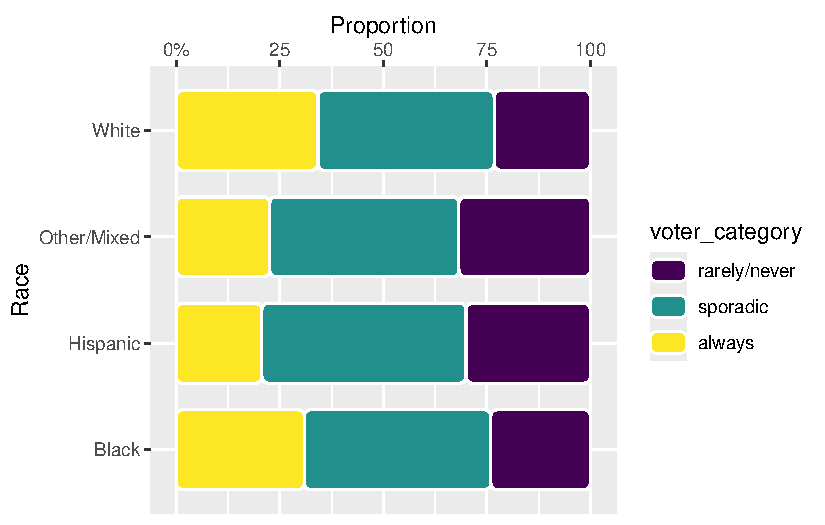
\includegraphics{Lab4_multinom_Questions-1_files/figure-pdf/unnamed-chunk-6-1.pdf}

\begin{Shaded}
\begin{Highlighting}[]
\CommentTok{\# Enter code}
\NormalTok{voter\_gender }\OtherTok{\textless{}{-}}\NormalTok{ voter\_data }\SpecialCharTok{\%\textgreater{}\%}
  \FunctionTok{count}\NormalTok{(gender, voter\_category) }\SpecialCharTok{\%\textgreater{}\%}
  \FunctionTok{mutate}\NormalTok{(}\AttributeTok{proportion =}\NormalTok{ n }\SpecialCharTok{/} \FunctionTok{sum}\NormalTok{(n))}

\NormalTok{plt\_gender }\OtherTok{=}\NormalTok{ voter\_gender }\SpecialCharTok{\%\textgreater{}\%}
  \FunctionTok{ggplot}\NormalTok{(}\FunctionTok{aes}\NormalTok{(}\AttributeTok{x=}\NormalTok{gender, }\AttributeTok{y=}\NormalTok{proportion, }\AttributeTok{group =}\NormalTok{ voter\_category, }\AttributeTok{fill =}\NormalTok{ voter\_category)) }\SpecialCharTok{+}
  \FunctionTok{geom\_chicklet}\NormalTok{(}\AttributeTok{width =} \FloatTok{0.75}\NormalTok{, }\AttributeTok{position=}\StringTok{"fill"}\NormalTok{)  }\SpecialCharTok{+} 
  \FunctionTok{scale\_y\_continuous}\NormalTok{(}
    \AttributeTok{expand =} \FunctionTok{c}\NormalTok{(}\DecValTok{0}\NormalTok{, }\FloatTok{0.0625}\NormalTok{),}
    \AttributeTok{position =} \StringTok{"right"}\NormalTok{,}
    \AttributeTok{breaks =} \FunctionTok{seq}\NormalTok{(}\DecValTok{0}\NormalTok{, }\DecValTok{1}\NormalTok{, }\FloatTok{0.25}\NormalTok{),}
    \AttributeTok{labels =} \FunctionTok{c}\NormalTok{(}\StringTok{"0\%"}\NormalTok{, }\FunctionTok{seq}\NormalTok{(}\DecValTok{25}\NormalTok{, }\DecValTok{100}\NormalTok{, }\DecValTok{25}\NormalTok{))}
\NormalTok{  ) }\SpecialCharTok{+}
  \FunctionTok{coord\_flip}\NormalTok{() }\SpecialCharTok{+} 
  \FunctionTok{labs}\NormalTok{(}\AttributeTok{x=}\StringTok{"Gender"}\NormalTok{, }\AttributeTok{y=}\StringTok{"Proportion"}\NormalTok{)}
\NormalTok{plt\_gender}
\end{Highlighting}
\end{Shaded}

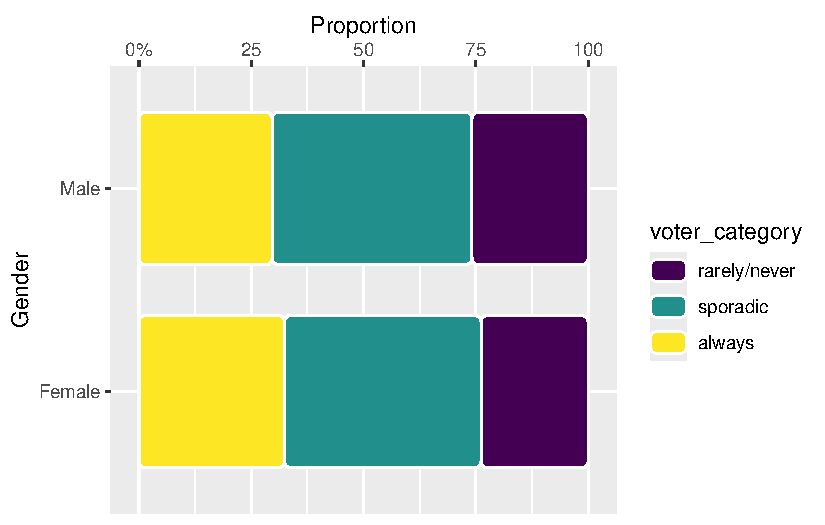
\includegraphics{Lab4_multinom_Questions-1_files/figure-pdf/unnamed-chunk-7-1.pdf}

The plots can be combined into a single plot using the patchwork
package.

\begin{Shaded}
\begin{Highlighting}[]
\FunctionTok{library}\NormalTok{(patchwork)}
\NormalTok{plt\_race }\SpecialCharTok{/}\NormalTok{ plt\_gender}
\end{Highlighting}
\end{Shaded}

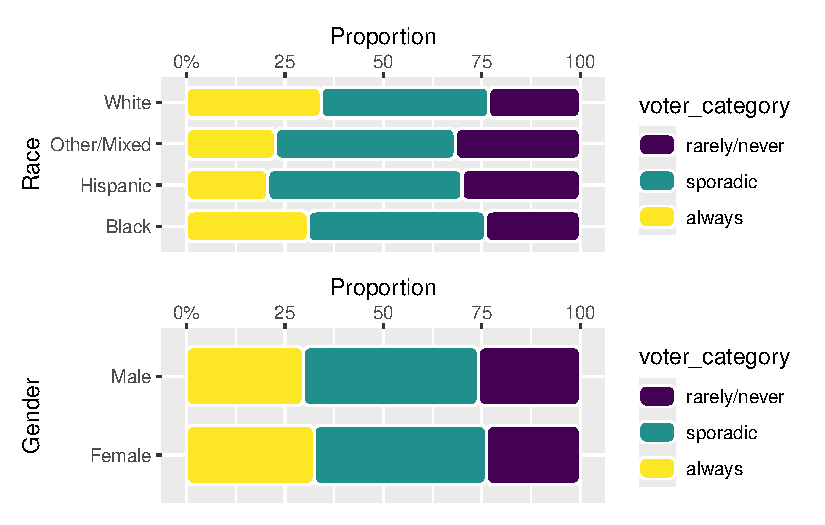
\includegraphics{Lab4_multinom_Questions-1_files/figure-pdf/unnamed-chunk-8-1.pdf}

\begin{itemize}
\tightlist
\item
  Fit a model using mean-centered age, race, gender, income, and
  education to predict voter category. Show the code used to fit the
  model, but do \textbf{not} display the model output.
\end{itemize}

\begin{Shaded}
\begin{Highlighting}[]
\FunctionTok{library}\NormalTok{(nnet)}

\NormalTok{model }\OtherTok{=} \FunctionTok{multinom}\NormalTok{(voter\_category }\SpecialCharTok{\textasciitilde{}}\NormalTok{ ppage }\SpecialCharTok{+}\NormalTok{ race }\SpecialCharTok{+}\NormalTok{ gender }\SpecialCharTok{+}\NormalTok{ income\_cat }\SpecialCharTok{+}\NormalTok{ educ, }
                     \AttributeTok{data =}\NormalTok{ voter\_data)}
\end{Highlighting}
\end{Shaded}

\begin{verbatim}
# weights:  36 (22 variable)
initial  value 6411.501317 
iter  10 value 5869.948482
iter  20 value 5728.474131
final  value 5693.312867 
converged
\end{verbatim}

\begin{itemize}
\tightlist
\item
  \emph{Should party identification be added to the model?}
\item
  \#Hint: Use an anova test to make the determination
\end{itemize}

\begin{Shaded}
\begin{Highlighting}[]
\NormalTok{model2 }\OtherTok{=} \FunctionTok{multinom}\NormalTok{(voter\_category }\SpecialCharTok{\textasciitilde{}}\NormalTok{ ppage }\SpecialCharTok{+}\NormalTok{ race }\SpecialCharTok{+}\NormalTok{ gender }\SpecialCharTok{+}\NormalTok{ income\_cat }\SpecialCharTok{+}\NormalTok{ educ }\SpecialCharTok{+}\NormalTok{ pol\_ident\_new, }
                     \AttributeTok{data =}\NormalTok{ voter\_data)}
\end{Highlighting}
\end{Shaded}

\begin{verbatim}
# weights:  45 (28 variable)
initial  value 6411.501317 
iter  10 value 5818.012349
iter  20 value 5709.034111
iter  30 value 5621.228937
final  value 5616.390878 
converged
\end{verbatim}

\begin{Shaded}
\begin{Highlighting}[]
\FunctionTok{anova}\NormalTok{(model, model2) }\SpecialCharTok{\%\textgreater{}\%} 
  \FunctionTok{kable}\NormalTok{()}
\end{Highlighting}
\end{Shaded}

\begin{longtable}[]{@{}
  >{\raggedright\arraybackslash}p{(\columnwidth - 12\tabcolsep) * \real{0.5321}}
  >{\raggedleft\arraybackslash}p{(\columnwidth - 12\tabcolsep) * \real{0.0917}}
  >{\raggedleft\arraybackslash}p{(\columnwidth - 12\tabcolsep) * \real{0.1009}}
  >{\raggedright\arraybackslash}p{(\columnwidth - 12\tabcolsep) * \real{0.0642}}
  >{\raggedleft\arraybackslash}p{(\columnwidth - 12\tabcolsep) * \real{0.0550}}
  >{\raggedleft\arraybackslash}p{(\columnwidth - 12\tabcolsep) * \real{0.0826}}
  >{\raggedleft\arraybackslash}p{(\columnwidth - 12\tabcolsep) * \real{0.0734}}@{}}
\toprule\noalign{}
\begin{minipage}[b]{\linewidth}\raggedright
Model
\end{minipage} & \begin{minipage}[b]{\linewidth}\raggedleft
Resid. df
\end{minipage} & \begin{minipage}[b]{\linewidth}\raggedleft
Resid. Dev
\end{minipage} & \begin{minipage}[b]{\linewidth}\raggedright
Test
\end{minipage} & \begin{minipage}[b]{\linewidth}\raggedleft
Df
\end{minipage} & \begin{minipage}[b]{\linewidth}\raggedleft
LR stat.
\end{minipage} & \begin{minipage}[b]{\linewidth}\raggedleft
Pr(Chi)
\end{minipage} \\
\midrule\noalign{}
\endhead
\bottomrule\noalign{}
\endlastfoot
ppage + race + gender + income\_cat + educ & 11650 & 11386.63 & & NA &
NA & NA \\
ppage + race + gender + income\_cat + educ + pol\_ident\_new & 11644 &
11232.78 & 1 vs 2 & 6 & 153.844 & 0 \\
\end{longtable}

\begin{verbatim}
> #Enter answer based on your code: Yes, party identification should be included in the model
\end{verbatim}

\textbf{Use the model you select for the remainder of the assignment}.

\subsection{LRT}\label{lrt}

\begin{itemize}
\item
  Run the full model and report overall significance of each of the
  terms

\begin{Shaded}
\begin{Highlighting}[]
\NormalTok{car}\SpecialCharTok{::}\FunctionTok{Anova}\NormalTok{(model2) }\SpecialCharTok{\%\textgreater{}\%} 
  \FunctionTok{kable}\NormalTok{()}
\end{Highlighting}
\end{Shaded}

  \begin{longtable}[]{@{}lrrr@{}}
  \toprule\noalign{}
  & LR Chisq & Df & Pr(\textgreater Chisq) \\
  \midrule\noalign{}
  \endhead
  \bottomrule\noalign{}
  \endlastfoot
  ppage & 638.297213 & 2 & 0.000000 \\
  race & 52.651508 & 6 & 0.000000 \\
  gender & 6.027914 & 2 & 0.049097 \\
  income\_cat & 67.721466 & 6 & 0.000000 \\
  educ & 154.136763 & 4 & 0.000000 \\
  pol\_ident\_new & 153.843978 & 6 & 0.000000 \\
  \end{longtable}

  \begin{quote}
  \section{All the temrs: age, race, gender, income, education, and
  party identification are all significant in predicting voter
  category}\label{all-the-temrs-age-race-gender-income-education-and-party-identification-are-all-significant-in-predicting-voter-category}
  \end{quote}
\end{itemize}

\subsection{Marginal Effects Political Group -
Emmeans}\label{marginal-effects-political-group---emmeans}

\begin{Shaded}
\begin{Highlighting}[]
\CommentTok{\#Get estimated marginal means from the model}

\CommentTok{\#using }
\NormalTok{multinomial\_analysis }\OtherTok{\textless{}{-}} \FunctionTok{emmeans}\NormalTok{(model2, }\SpecialCharTok{\textasciitilde{}}\NormalTok{ pol\_ident\_new}\SpecialCharTok{|}\NormalTok{voter\_category)}

\NormalTok{coefs }\OtherTok{=} \FunctionTok{contrast}\NormalTok{(}\FunctionTok{regrid}\NormalTok{(multinomial\_analysis, }\StringTok{"log"}\NormalTok{),}\StringTok{"trt.vs.ctrl1"}\NormalTok{,  }\AttributeTok{by=}\StringTok{"pol\_ident\_new"}\NormalTok{)}
\CommentTok{\# you can add a parameter to the above command, ref = newbaseline, if you want to change baseline}

\FunctionTok{update}\NormalTok{(coefs, }\AttributeTok{by =} \StringTok{"contrast"}\NormalTok{) }\SpecialCharTok{\%\textgreater{}\%}
 \FunctionTok{kable}\NormalTok{(}\AttributeTok{format =} \StringTok{"markdown"}\NormalTok{, }\AttributeTok{digits =} \DecValTok{3}\NormalTok{)}
\end{Highlighting}
\end{Shaded}

\begin{longtable}[]{@{}
  >{\raggedright\arraybackslash}p{(\columnwidth - 12\tabcolsep) * \real{0.3514}}
  >{\raggedright\arraybackslash}p{(\columnwidth - 12\tabcolsep) * \real{0.1892}}
  >{\raggedleft\arraybackslash}p{(\columnwidth - 12\tabcolsep) * \real{0.1216}}
  >{\raggedleft\arraybackslash}p{(\columnwidth - 12\tabcolsep) * \real{0.0811}}
  >{\raggedleft\arraybackslash}p{(\columnwidth - 12\tabcolsep) * \real{0.0405}}
  >{\raggedleft\arraybackslash}p{(\columnwidth - 12\tabcolsep) * \real{0.1081}}
  >{\raggedleft\arraybackslash}p{(\columnwidth - 12\tabcolsep) * \real{0.1081}}@{}}
\toprule\noalign{}
\begin{minipage}[b]{\linewidth}\raggedright
contrast
\end{minipage} & \begin{minipage}[b]{\linewidth}\raggedright
pol\_ident\_new
\end{minipage} & \begin{minipage}[b]{\linewidth}\raggedleft
estimate
\end{minipage} & \begin{minipage}[b]{\linewidth}\raggedleft
SE
\end{minipage} & \begin{minipage}[b]{\linewidth}\raggedleft
df
\end{minipage} & \begin{minipage}[b]{\linewidth}\raggedleft
t.ratio
\end{minipage} & \begin{minipage}[b]{\linewidth}\raggedleft
p.value
\end{minipage} \\
\midrule\noalign{}
\endhead
\bottomrule\noalign{}
\endlastfoot
sporadic - (rarely/never) & Dem & 0.961 & 0.070 & 28 & 13.722 & 0.000 \\
always - (rarely/never) & Dem & 0.480 & 0.074 & 28 & 6.498 & 0.000 \\
sporadic - (rarely/never) & Indep & 0.591 & 0.077 & 28 & 7.643 &
0.000 \\
always - (rarely/never) & Indep & -0.049 & 0.084 & 28 & -0.590 &
0.900 \\
sporadic - (rarely/never) & Other & 0.078 & 0.087 & 28 & 0.902 &
0.747 \\
always - (rarely/never) & Other & -0.835 & 0.110 & 28 & -7.577 &
0.000 \\
sporadic - (rarely/never) & Rep & 0.883 & 0.084 & 28 & 10.469 & 0.000 \\
always - (rarely/never) & Rep & 0.327 & 0.089 & 28 & 3.672 & 0.004 \\
\end{longtable}

\subsection{Marginal Effects of Education -
Emmeans}\label{marginal-effects-of-education---emmeans}

\begin{Shaded}
\begin{Highlighting}[]
\CommentTok{\#Get estimated marginal means from the model}

\CommentTok{\#using }
\NormalTok{multinomial\_analysis }\OtherTok{\textless{}{-}} \FunctionTok{emmeans}\NormalTok{(model2, }\SpecialCharTok{\textasciitilde{}}\NormalTok{ educ}\SpecialCharTok{|}\NormalTok{voter\_category)}

\NormalTok{coefs }\OtherTok{=} \FunctionTok{contrast}\NormalTok{(}\FunctionTok{regrid}\NormalTok{(multinomial\_analysis, }\StringTok{"log"}\NormalTok{),}\StringTok{"trt.vs.ctrl1"}\NormalTok{,  }\AttributeTok{by=}\StringTok{"educ"}\NormalTok{)}
\CommentTok{\# you can add a parameter to the above command, ref = newbaseline, if you want to change baseline}

\FunctionTok{update}\NormalTok{(coefs, }\AttributeTok{by =} \StringTok{"contrast"}\NormalTok{) }\SpecialCharTok{\%\textgreater{}\%}
 \FunctionTok{kable}\NormalTok{(}\AttributeTok{format =} \StringTok{"markdown"}\NormalTok{, }\AttributeTok{digits =} \DecValTok{3}\NormalTok{)}
\end{Highlighting}
\end{Shaded}

\begin{longtable}[]{@{}
  >{\raggedright\arraybackslash}p{(\columnwidth - 12\tabcolsep) * \real{0.3250}}
  >{\raggedright\arraybackslash}p{(\columnwidth - 12\tabcolsep) * \real{0.2500}}
  >{\raggedleft\arraybackslash}p{(\columnwidth - 12\tabcolsep) * \real{0.1125}}
  >{\raggedleft\arraybackslash}p{(\columnwidth - 12\tabcolsep) * \real{0.0750}}
  >{\raggedleft\arraybackslash}p{(\columnwidth - 12\tabcolsep) * \real{0.0375}}
  >{\raggedleft\arraybackslash}p{(\columnwidth - 12\tabcolsep) * \real{0.1000}}
  >{\raggedleft\arraybackslash}p{(\columnwidth - 12\tabcolsep) * \real{0.1000}}@{}}
\toprule\noalign{}
\begin{minipage}[b]{\linewidth}\raggedright
contrast
\end{minipage} & \begin{minipage}[b]{\linewidth}\raggedright
educ
\end{minipage} & \begin{minipage}[b]{\linewidth}\raggedleft
estimate
\end{minipage} & \begin{minipage}[b]{\linewidth}\raggedleft
SE
\end{minipage} & \begin{minipage}[b]{\linewidth}\raggedleft
df
\end{minipage} & \begin{minipage}[b]{\linewidth}\raggedleft
t.ratio
\end{minipage} & \begin{minipage}[b]{\linewidth}\raggedleft
p.value
\end{minipage} \\
\midrule\noalign{}
\endhead
\bottomrule\noalign{}
\endlastfoot
sporadic - (rarely/never) & College & 0.986 & 0.076 & 28 & 12.904 &
0.000 \\
always - (rarely/never) & College & 0.477 & 0.080 & 28 & 5.960 &
0.000 \\
sporadic - (rarely/never) & High school or less & 0.187 & 0.069 & 28 &
2.705 & 0.031 \\
always - (rarely/never) & High school or less & -0.711 & 0.080 & 28 &
-8.883 & 0.000 \\
sporadic - (rarely/never) & Some college & 0.707 & 0.074 & 28 & 9.512 &
0.000 \\
always - (rarely/never) & Some college & 0.167 & 0.079 & 28 & 2.114 &
0.112 \\
\end{longtable}

\begin{itemize}
\tightlist
\item
  Next, plot the predicted probabilities of voter category as a function
  of Age and Party ID
\end{itemize}

\begin{Shaded}
\begin{Highlighting}[]
  \FunctionTok{ggemmeans}\NormalTok{(model2, }\AttributeTok{terms =} \FunctionTok{c}\NormalTok{(}\StringTok{"ppage"}\NormalTok{)) }\SpecialCharTok{\%\textgreater{}\%} 
      \FunctionTok{ggplot}\NormalTok{(., }\FunctionTok{aes}\NormalTok{(}\AttributeTok{x =}\NormalTok{ x, }\AttributeTok{y =}\NormalTok{ predicted, }\AttributeTok{fill =}\NormalTok{ response.level)) }\SpecialCharTok{+}
      \FunctionTok{geom\_area}\NormalTok{() }\SpecialCharTok{+} 
      \FunctionTok{geom\_rug}\NormalTok{(}\AttributeTok{sides =} \StringTok{"b"}\NormalTok{, }\AttributeTok{position =} \StringTok{"jitter"}\NormalTok{, }\AttributeTok{alpha =}\NormalTok{ .}\DecValTok{5}\NormalTok{) }\SpecialCharTok{+} 
      \FunctionTok{labs}\NormalTok{(}\AttributeTok{x =} \StringTok{"}\SpecialCharTok{\textbackslash{}n}\StringTok{Age"}\NormalTok{, }\AttributeTok{y =} \StringTok{"Predicted Probablity}\SpecialCharTok{\textbackslash{}n}\StringTok{"}\NormalTok{, }\AttributeTok{title =} \StringTok{"Predicted Probabilities of Voting Frequency by Age"}\NormalTok{) }\SpecialCharTok{+}
      \FunctionTok{scale\_fill\_manual}\NormalTok{(}
        \AttributeTok{name =} \ConstantTok{NULL}\NormalTok{,}
        \AttributeTok{values =} \FunctionTok{c}\NormalTok{(}\StringTok{"always"} \OtherTok{=} \StringTok{"\#F6B533"}\NormalTok{, }\StringTok{"sporadic"} \OtherTok{=} \StringTok{"\#D07EA2"}\NormalTok{, }\StringTok{"rarely/never"} \OtherTok{=} \StringTok{"\#9854F7"}\NormalTok{),}
        \AttributeTok{labels =} \FunctionTok{c}\NormalTok{(}\StringTok{"RARELY OR NEVER VOTE    "}\NormalTok{, }\StringTok{"SOMETIMES VOTE    "}\NormalTok{, }\StringTok{"ALMOST ALWAYS VOTE    "}\NormalTok{),}
        \AttributeTok{breaks =} \FunctionTok{c}\NormalTok{(}\StringTok{"rarely/never"}\NormalTok{, }\StringTok{"sporadic"}\NormalTok{, }\StringTok{"always"}\NormalTok{)}
\NormalTok{      ) }\SpecialCharTok{+}
      \FunctionTok{theme\_minimal}\NormalTok{()}
\end{Highlighting}
\end{Shaded}

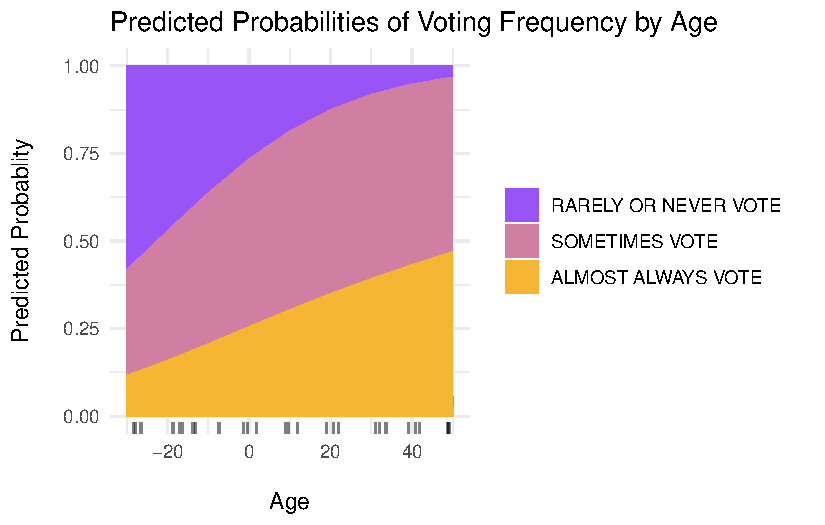
\includegraphics{Lab4_multinom_Questions-1_files/figure-pdf/unnamed-chunk-14-1.pdf}

\begin{Shaded}
\begin{Highlighting}[]
 \FunctionTok{ggemmeans}\NormalTok{(model2, }\AttributeTok{terms=}\FunctionTok{c}\NormalTok{(}\StringTok{"pol\_ident\_new"}\NormalTok{)) }\SpecialCharTok{\%\textgreater{}\%}   \FunctionTok{ggplot}\NormalTok{(., }\FunctionTok{aes}\NormalTok{(}\AttributeTok{x =}\NormalTok{ x, }\AttributeTok{y =}\NormalTok{ predicted, }\AttributeTok{fill =}\NormalTok{ response.level)) }\SpecialCharTok{+} 
  \FunctionTok{geom\_bar}\NormalTok{(}\AttributeTok{stat =} \StringTok{"identity"}\NormalTok{ ) }\SpecialCharTok{+}
    \FunctionTok{geom\_text}\NormalTok{(}\FunctionTok{aes}\NormalTok{(}\AttributeTok{label =} \FunctionTok{round}\NormalTok{(predicted, }\DecValTok{3}\NormalTok{)), }\AttributeTok{color=}\StringTok{"white"}\NormalTok{, }\AttributeTok{position =} \FunctionTok{position\_fill}\NormalTok{(}\AttributeTok{vjust =} \FloatTok{0.5}\NormalTok{),}\AttributeTok{size=}\DecValTok{3}\NormalTok{)  }\SpecialCharTok{+} 
  \FunctionTok{labs}\NormalTok{(}\AttributeTok{x=}\StringTok{"Education"}\NormalTok{, }\AttributeTok{y=}\StringTok{"Predicted Probablity"}\NormalTok{) }\SpecialCharTok{+} 
  \FunctionTok{theme}\NormalTok{(}\AttributeTok{text =} \FunctionTok{element\_text}\NormalTok{(}\AttributeTok{size =} \DecValTok{30}\NormalTok{)) }\SpecialCharTok{+}  
  \FunctionTok{scale\_fill\_viridis}\NormalTok{(}\AttributeTok{discrete =} \ConstantTok{TRUE}\NormalTok{) }\SpecialCharTok{+} 
  \FunctionTok{theme\_lucid}\NormalTok{(}\AttributeTok{base\_size=}\DecValTok{25}\NormalTok{)}
\end{Highlighting}
\end{Shaded}

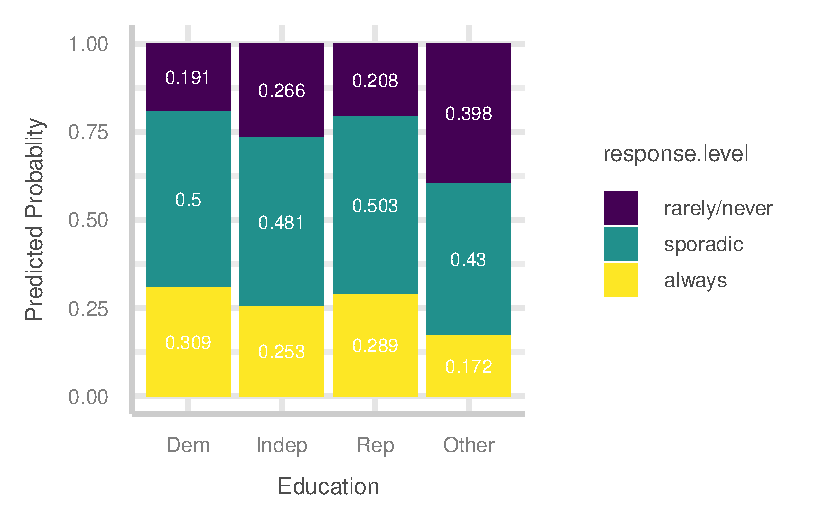
\includegraphics{Lab4_multinom_Questions-1_files/figure-pdf/unnamed-chunk-14-2.pdf}

Plot predicted probabilities as a function of education and voting
frequency.

\begin{Shaded}
\begin{Highlighting}[]
 \FunctionTok{ggemmeans}\NormalTok{(model2, }\AttributeTok{terms=}\FunctionTok{c}\NormalTok{(}\StringTok{"educ"}\NormalTok{)) }\SpecialCharTok{\%\textgreater{}\%} \FunctionTok{ggplot}\NormalTok{(., }\FunctionTok{aes}\NormalTok{(}\AttributeTok{x =}\NormalTok{ x, }\AttributeTok{y =}\NormalTok{ predicted, }\AttributeTok{fill =}\NormalTok{ response.level)) }\SpecialCharTok{+} 
  \FunctionTok{geom\_bar}\NormalTok{(}\AttributeTok{stat =} \StringTok{"identity"}\NormalTok{ ) }\SpecialCharTok{+}
    \FunctionTok{geom\_text}\NormalTok{(}\FunctionTok{aes}\NormalTok{(}\AttributeTok{label =} \FunctionTok{round}\NormalTok{(predicted, }\DecValTok{3}\NormalTok{)), }\AttributeTok{color=}\StringTok{"white"}\NormalTok{, }\AttributeTok{position =} \FunctionTok{position\_fill}\NormalTok{(}\AttributeTok{vjust =} \FloatTok{0.5}\NormalTok{),}\AttributeTok{size=}\DecValTok{3}\NormalTok{)  }\SpecialCharTok{+} 
  \FunctionTok{labs}\NormalTok{(}\AttributeTok{x=}\StringTok{"Education"}\NormalTok{, }\AttributeTok{y=}\StringTok{"Predicted Probablity"}\NormalTok{) }\SpecialCharTok{+} 
  \FunctionTok{theme}\NormalTok{(}\AttributeTok{text =} \FunctionTok{element\_text}\NormalTok{(}\AttributeTok{size =} \DecValTok{30}\NormalTok{)) }\SpecialCharTok{+}  
  \FunctionTok{scale\_fill\_viridis}\NormalTok{(}\AttributeTok{discrete =} \ConstantTok{TRUE}\NormalTok{) }\SpecialCharTok{+} 
  \FunctionTok{theme\_lucid}\NormalTok{(}\AttributeTok{base\_size=}\DecValTok{25}\NormalTok{)}
\end{Highlighting}
\end{Shaded}

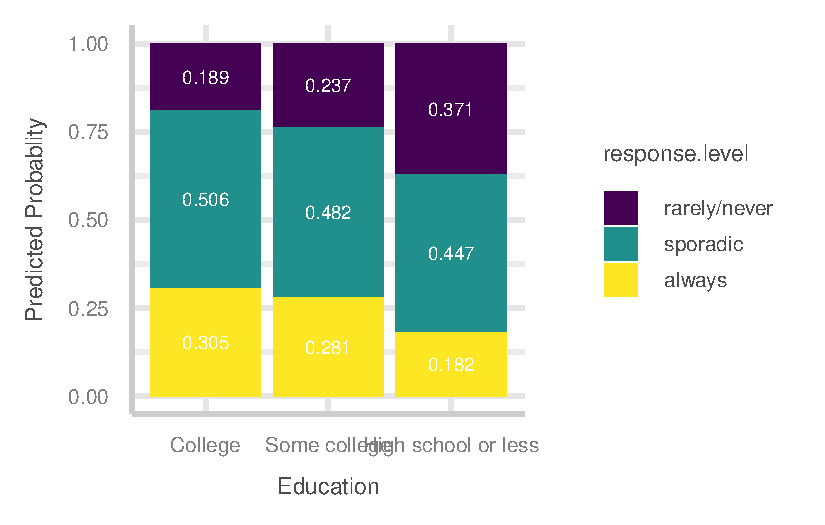
\includegraphics{Lab4_multinom_Questions-1_files/figure-pdf/unnamed-chunk-15-1.pdf}

\subsection{Write-up}\label{write-up}

\subsubsection{Differences between political groups and voting behavior
-
Emmeans}\label{differences-between-political-groups-and-voting-behavior---emmeans}

\begin{Shaded}
\begin{Highlighting}[]
\NormalTok{multinomial\_analysis }\OtherTok{\textless{}{-}} \FunctionTok{emmeans}\NormalTok{(model2, }\SpecialCharTok{\textasciitilde{}}\NormalTok{ pol\_ident\_new}\SpecialCharTok{|}\NormalTok{voter\_category)}

\NormalTok{coefs }\OtherTok{=} \FunctionTok{contrast}\NormalTok{(}\FunctionTok{regrid}\NormalTok{(multinomial\_analysis, }\StringTok{"log"}\NormalTok{),}\StringTok{"trt.vs.ctrl1"}\NormalTok{,  }\AttributeTok{by=}\StringTok{"pol\_ident\_new"}\NormalTok{)}
\CommentTok{\# you can add a parameter to the above command, ref = newbaseline, if you want to change baseline}

\FunctionTok{update}\NormalTok{(coefs, }\AttributeTok{by =} \StringTok{"contrast"}\NormalTok{) }\SpecialCharTok{\%\textgreater{}\%}
 \FunctionTok{kable}\NormalTok{(}\AttributeTok{format =} \StringTok{"markdown"}\NormalTok{, }\AttributeTok{digits =} \DecValTok{3}\NormalTok{)}
\end{Highlighting}
\end{Shaded}

\begin{longtable}[]{@{}
  >{\raggedright\arraybackslash}p{(\columnwidth - 12\tabcolsep) * \real{0.3514}}
  >{\raggedright\arraybackslash}p{(\columnwidth - 12\tabcolsep) * \real{0.1892}}
  >{\raggedleft\arraybackslash}p{(\columnwidth - 12\tabcolsep) * \real{0.1216}}
  >{\raggedleft\arraybackslash}p{(\columnwidth - 12\tabcolsep) * \real{0.0811}}
  >{\raggedleft\arraybackslash}p{(\columnwidth - 12\tabcolsep) * \real{0.0405}}
  >{\raggedleft\arraybackslash}p{(\columnwidth - 12\tabcolsep) * \real{0.1081}}
  >{\raggedleft\arraybackslash}p{(\columnwidth - 12\tabcolsep) * \real{0.1081}}@{}}
\toprule\noalign{}
\begin{minipage}[b]{\linewidth}\raggedright
contrast
\end{minipage} & \begin{minipage}[b]{\linewidth}\raggedright
pol\_ident\_new
\end{minipage} & \begin{minipage}[b]{\linewidth}\raggedleft
estimate
\end{minipage} & \begin{minipage}[b]{\linewidth}\raggedleft
SE
\end{minipage} & \begin{minipage}[b]{\linewidth}\raggedleft
df
\end{minipage} & \begin{minipage}[b]{\linewidth}\raggedleft
t.ratio
\end{minipage} & \begin{minipage}[b]{\linewidth}\raggedleft
p.value
\end{minipage} \\
\midrule\noalign{}
\endhead
\bottomrule\noalign{}
\endlastfoot
sporadic - (rarely/never) & Dem & 0.961 & 0.070 & 28 & 13.722 & 0.000 \\
always - (rarely/never) & Dem & 0.480 & 0.074 & 28 & 6.498 & 0.000 \\
sporadic - (rarely/never) & Indep & 0.591 & 0.077 & 28 & 7.643 &
0.000 \\
always - (rarely/never) & Indep & -0.049 & 0.084 & 28 & -0.590 &
0.900 \\
sporadic - (rarely/never) & Other & 0.078 & 0.087 & 28 & 0.902 &
0.747 \\
always - (rarely/never) & Other & -0.835 & 0.110 & 28 & -7.577 &
0.000 \\
sporadic - (rarely/never) & Rep & 0.883 & 0.084 & 28 & 10.469 & 0.000 \\
always - (rarely/never) & Rep & 0.327 & 0.089 & 28 & 3.672 & 0.004 \\
\end{longtable}

\begin{Shaded}
\begin{Highlighting}[]
\CommentTok{\# get difference between yes{-}no and fair{-}excellent}
\FunctionTok{contrast}\NormalTok{(coefs, }\StringTok{"revpairwise"}\NormalTok{, }\AttributeTok{by =} \StringTok{"contrast"}\NormalTok{) }\SpecialCharTok{\%\textgreater{}\%}
  \FunctionTok{kable}\NormalTok{(}\AttributeTok{format =} \StringTok{"markdown"}\NormalTok{, }\AttributeTok{digits =} \DecValTok{3}\NormalTok{)}
\end{Highlighting}
\end{Shaded}

\begin{longtable}[]{@{}
  >{\raggedright\arraybackslash}p{(\columnwidth - 12\tabcolsep) * \real{0.1892}}
  >{\raggedright\arraybackslash}p{(\columnwidth - 12\tabcolsep) * \real{0.3514}}
  >{\raggedleft\arraybackslash}p{(\columnwidth - 12\tabcolsep) * \real{0.1216}}
  >{\raggedleft\arraybackslash}p{(\columnwidth - 12\tabcolsep) * \real{0.0811}}
  >{\raggedleft\arraybackslash}p{(\columnwidth - 12\tabcolsep) * \real{0.0405}}
  >{\raggedleft\arraybackslash}p{(\columnwidth - 12\tabcolsep) * \real{0.1081}}
  >{\raggedleft\arraybackslash}p{(\columnwidth - 12\tabcolsep) * \real{0.1081}}@{}}
\toprule\noalign{}
\begin{minipage}[b]{\linewidth}\raggedright
contrast1
\end{minipage} & \begin{minipage}[b]{\linewidth}\raggedright
contrast
\end{minipage} & \begin{minipage}[b]{\linewidth}\raggedleft
estimate
\end{minipage} & \begin{minipage}[b]{\linewidth}\raggedleft
SE
\end{minipage} & \begin{minipage}[b]{\linewidth}\raggedleft
df
\end{minipage} & \begin{minipage}[b]{\linewidth}\raggedleft
t.ratio
\end{minipage} & \begin{minipage}[b]{\linewidth}\raggedleft
p.value
\end{minipage} \\
\midrule\noalign{}
\endhead
\bottomrule\noalign{}
\endlastfoot
Indep - Dem & sporadic - (rarely/never) & -0.370 & 0.094 & 28 & -3.933 &
0.003 \\
Other - Dem & sporadic - (rarely/never) & -0.883 & 0.103 & 28 & -8.578 &
0.000 \\
Other - Indep & sporadic - (rarely/never) & -0.513 & 0.107 & 28 & -4.807
& 0.000 \\
Rep - Dem & sporadic - (rarely/never) & -0.078 & 0.099 & 28 & -0.787 &
0.860 \\
Rep - Indep & sporadic - (rarely/never) & 0.292 & 0.099 & 28 & 2.965 &
0.029 \\
Rep - Other & sporadic - (rarely/never) & 0.805 & 0.109 & 28 & 7.404 &
0.000 \\
Indep - Dem & always - (rarely/never) & -0.529 & 0.101 & 28 & -5.255 &
0.000 \\
Other - Dem & always - (rarely/never) & -1.315 & 0.125 & 28 & -10.508 &
0.000 \\
Other - Indep & always - (rarely/never) & -0.786 & 0.129 & 28 & -6.072 &
0.000 \\
Rep - Dem & always - (rarely/never) & -0.153 & 0.104 & 28 & -1.470 &
0.468 \\
Rep - Indep & always - (rarely/never) & 0.376 & 0.104 & 28 & 3.605 &
0.006 \\
Rep - Other & always - (rarely/never) & 1.162 & 0.130 & 28 & 8.969 &
0.000 \\
\end{longtable}

Enter your interpretation here:

Voters who are Democrats are 2.61 times more likely to vote sporadically
than vote rarely/never.

Voters who are Democrats are 1.62 times more likely to vote always than
vote rarely/never.

Voters who are Independents are 1.81 times more likely to vote
sporadically than vote rarely/never.

Voters who are Independents are 4.78\% less likely to vote always than
vote rarely/never.

Voters who belong to other political parties are 1.08 times more likely
to vote sporadically than vote rarely/never.

Voters who belong to other political parties are 56.61\% less likely to
vote always than vote rarely/never.

Voters who are Republicans are 2.42 times more likely to vote
sporadically than vote rarely/never.

Voters who are Republicans are 1.39 times more likely to vote always
than vote rarely/never.

Voters who are Independents are 30.93\% less likely to vote sporadically
than vote rarely/never compared to voters who are Democrats.

Voters who belong to voters who belong to other political parties are
58.65\% less likely to vote sporadically than vote rarely/never compared
to voters who are Democrats.

Voters who belong to other political parties are 40.13\% less likely to
vote sporadically than vote rarely/never compared to voters who are
Republicans.

Voters who are Republicans are 7.50\% less likely to vote sporadically
than vote rarely/never compared to voters who are Democrats.

Voters who are Republicans are 1.34 times more likely to vote
sporadically than vote rarely/never compared to voters who are
Independents.

Voters who are Republicans are 2.24 times more likely to vote
sporadically than vote rarely/never compared to voters who belong to
other political parties.

Voters who are Independents are 41.08\% less likely to vote always than
vote rarely/never compared to voters who are Democrats.

Voters who belong to other political parties are 73.15\% less likely to
vote always than vote rarely/never compared to voters who are Democrats.

Voters who belong to other political parties are 54.43\% less likely to
vote always than vote rarely/never compared to voters who are
Republicans.

Voters who are Republicans are 14.19\% less likely to vote always than
vote rarely/never compared to voters who are Democrats.

Voters who are Republicans are 1.46 times more likely to vote always
than vote rarely/never compared to voters who are Independents.

Voters who are Republicans are 3.20 times more likely to vote always
than vote rarely/never compared to voters who belong to other political
parties.

\subsubsection{Differences between education level and voting behavior -
Emmeans}\label{differences-between-education-level-and-voting-behavior---emmeans}

Last part of the assignment: Interpret the results from running the
following code for your model

\begin{Shaded}
\begin{Highlighting}[]
\NormalTok{multi\_an }\OtherTok{\textless{}{-}} \FunctionTok{emmeans}\NormalTok{(model, }\SpecialCharTok{\textasciitilde{}}\NormalTok{ educ}\SpecialCharTok{|}\NormalTok{voter\_category)}

\NormalTok{coefs }\OtherTok{=} \FunctionTok{contrast}\NormalTok{(}\FunctionTok{regrid}\NormalTok{(multi\_an, }\StringTok{"log"}\NormalTok{),}\StringTok{"trt.vs.ctrl1"}\NormalTok{,  }\AttributeTok{by=}\StringTok{"educ"}\NormalTok{)}

\FunctionTok{update}\NormalTok{(coefs, }\AttributeTok{by =} \StringTok{"contrast"}\NormalTok{) }\SpecialCharTok{\%\textgreater{}\%} 
  \FunctionTok{kable}\NormalTok{(}\AttributeTok{format =} \StringTok{"markdown"}\NormalTok{, }\AttributeTok{digits =} \DecValTok{3}\NormalTok{)}
\end{Highlighting}
\end{Shaded}

\begin{longtable}[]{@{}
  >{\raggedright\arraybackslash}p{(\columnwidth - 12\tabcolsep) * \real{0.3250}}
  >{\raggedright\arraybackslash}p{(\columnwidth - 12\tabcolsep) * \real{0.2500}}
  >{\raggedleft\arraybackslash}p{(\columnwidth - 12\tabcolsep) * \real{0.1125}}
  >{\raggedleft\arraybackslash}p{(\columnwidth - 12\tabcolsep) * \real{0.0750}}
  >{\raggedleft\arraybackslash}p{(\columnwidth - 12\tabcolsep) * \real{0.0375}}
  >{\raggedleft\arraybackslash}p{(\columnwidth - 12\tabcolsep) * \real{0.1000}}
  >{\raggedleft\arraybackslash}p{(\columnwidth - 12\tabcolsep) * \real{0.1000}}@{}}
\toprule\noalign{}
\begin{minipage}[b]{\linewidth}\raggedright
contrast
\end{minipage} & \begin{minipage}[b]{\linewidth}\raggedright
educ
\end{minipage} & \begin{minipage}[b]{\linewidth}\raggedleft
estimate
\end{minipage} & \begin{minipage}[b]{\linewidth}\raggedleft
SE
\end{minipage} & \begin{minipage}[b]{\linewidth}\raggedleft
df
\end{minipage} & \begin{minipage}[b]{\linewidth}\raggedleft
t.ratio
\end{minipage} & \begin{minipage}[b]{\linewidth}\raggedleft
p.value
\end{minipage} \\
\midrule\noalign{}
\endhead
\bottomrule\noalign{}
\endlastfoot
sporadic - (rarely/never) & College & 1.156 & 0.075 & 22 & 15.483 &
0.000 \\
always - (rarely/never) & College & 0.711 & 0.079 & 22 & 9.041 &
0.000 \\
sporadic - (rarely/never) & High school or less & 0.259 & 0.069 & 22 &
3.749 & 0.003 \\
always - (rarely/never) & High school or less & -0.602 & 0.081 & 22 &
-7.476 & 0.000 \\
sporadic - (rarely/never) & Some college & 0.806 & 0.075 & 22 & 10.818 &
0.000 \\
always - (rarely/never) & Some college & 0.311 & 0.080 & 22 & 3.895 &
0.002 \\
\end{longtable}

\begin{Shaded}
\begin{Highlighting}[]
\CommentTok{\# get difference between yes{-}no and fair{-}excellent}
\FunctionTok{contrast}\NormalTok{(coefs, }\StringTok{"revpairwise"}\NormalTok{, }\AttributeTok{by =} \StringTok{"contrast"}\NormalTok{) }\SpecialCharTok{\%\textgreater{}\%}
  \FunctionTok{kable}\NormalTok{(}\AttributeTok{format =} \StringTok{"markdown"}\NormalTok{, }\AttributeTok{digits =} \DecValTok{3}\NormalTok{)}
\end{Highlighting}
\end{Shaded}

\begin{longtable}[]{@{}
  >{\raggedright\arraybackslash}p{(\columnwidth - 12\tabcolsep) * \real{0.3684}}
  >{\raggedright\arraybackslash}p{(\columnwidth - 12\tabcolsep) * \real{0.2737}}
  >{\raggedleft\arraybackslash}p{(\columnwidth - 12\tabcolsep) * \real{0.0947}}
  >{\raggedleft\arraybackslash}p{(\columnwidth - 12\tabcolsep) * \real{0.0632}}
  >{\raggedleft\arraybackslash}p{(\columnwidth - 12\tabcolsep) * \real{0.0316}}
  >{\raggedleft\arraybackslash}p{(\columnwidth - 12\tabcolsep) * \real{0.0842}}
  >{\raggedleft\arraybackslash}p{(\columnwidth - 12\tabcolsep) * \real{0.0842}}@{}}
\toprule\noalign{}
\begin{minipage}[b]{\linewidth}\raggedright
contrast1
\end{minipage} & \begin{minipage}[b]{\linewidth}\raggedright
contrast
\end{minipage} & \begin{minipage}[b]{\linewidth}\raggedleft
estimate
\end{minipage} & \begin{minipage}[b]{\linewidth}\raggedleft
SE
\end{minipage} & \begin{minipage}[b]{\linewidth}\raggedleft
df
\end{minipage} & \begin{minipage}[b]{\linewidth}\raggedleft
t.ratio
\end{minipage} & \begin{minipage}[b]{\linewidth}\raggedleft
p.value
\end{minipage} \\
\midrule\noalign{}
\endhead
\bottomrule\noalign{}
\endlastfoot
High school or less - College & sporadic - (rarely/never) & -0.897 &
0.095 & 22 & -9.409 & 0.000 \\
Some college - College & sporadic - (rarely/never) & -0.349 & 0.092 & 22
& -3.779 & 0.003 \\
Some college - High school or less & sporadic - (rarely/never) & 0.547 &
0.089 & 22 & 6.162 & 0.000 \\
High school or less - College & always - (rarely/never) & -1.313 & 0.105
& 22 & -12.463 & 0.000 \\
Some college - College & always - (rarely/never) & -0.401 & 0.098 & 22 &
-4.091 & 0.001 \\
Some college - High school or less & always - (rarely/never) & 0.913 &
0.099 & 22 & 9.206 & 0.000 \\
\end{longtable}

Enter your interpretation here:

Voters with a highest degree of college are 3.18 times more likely to
vote sporadically than vote rarely/never.

Voters with a highest degree of college are 2.04 times more likely to
vote always than vote rarely/never.

Voters with a highest degree of high school or less are 1.30 times more
likely to vote sporadically than vote rarely/never.

Voters with a highest degree of high school or less are 45.23\% less
likely to vote always than vote rarely/never.

Voters with a highest degree of some college are 2.24 times more likely
to vote sporadically than vote rarely/never.

Voters with a highest degree of some college are 1.36 times more likely
to vote always than vote rarely/never.

Voters with a highest degree of high school or less are 59.22\% less
likely to vote sporadically than vote rarely/never compared to voters
with a highest degree of college.

Voters with a highest degree of some college are 29.46\% less likely to
vote sporadically than vote rarely/never compared to voters with a
highest degree of college.

Voters with a highest degree of some college are 1.73 times more likely
to vote sporadically than vote rarely/never compared to voters with a
highest degree of high school or less.

Voters with a highest degree of high school or less are 73.10\% less
likely to vote always than vote rarely/never compared to voters with a
highest degree of college.

Voters with a highest degree of some college are 33.03\% less likely to
vote always than vote rarely/never compared to voters with a highest
degree of college.

Voters with a highest degree of some college are 2.49 times more likely
to vote always than vote rarely/never compared to voters with a highest
degree of high school or less.



\end{document}
